\chapter{Conclusioni}
Com'è stato possibile notare dal capitolo precedente,
l'algoritmo che con un budget di tempo $\mathcal{B}$ limitato è riuscito a trovare
il risultato migliore, è stato Increase Search.
Di seguente riportiamo alcune considerazioni maturate
dallo studio del modello di ranking e del caso sperimentale.

\subsection{Andamento dei valori}
Il grafico sottostante illustra sull'asse delle ordinate il valore assunto
dalla componente $i$-esima del vettore dei pesi.

\begin{figure}[h!]
	\centering
	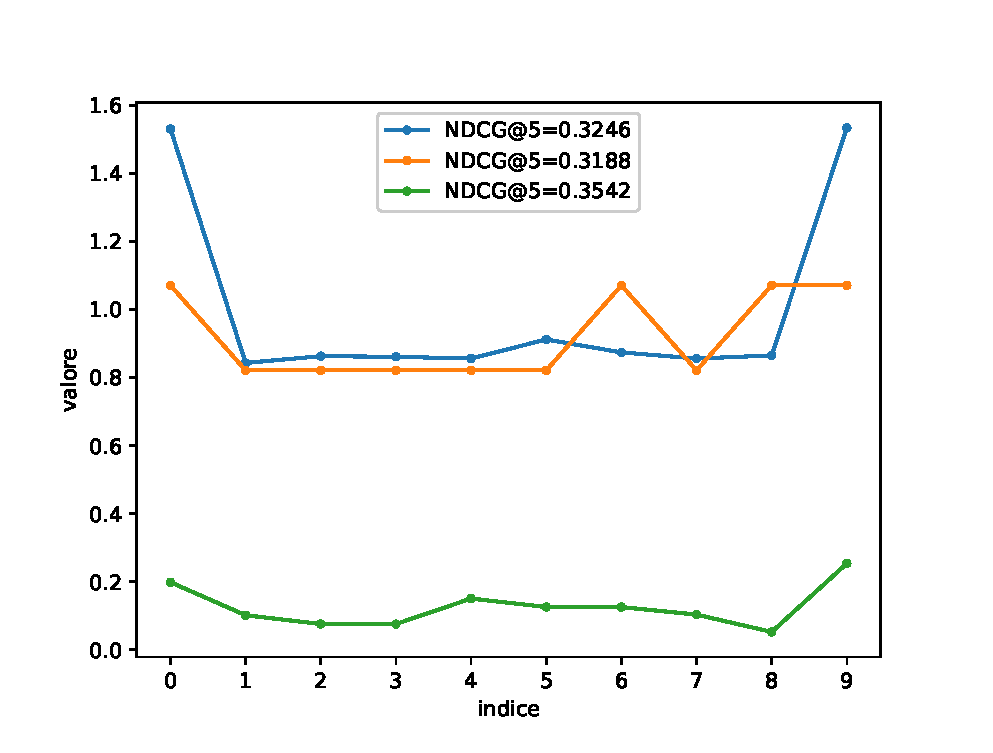
\includegraphics[width=0.7\linewidth]{figure/w_vectors}
	\caption[Distribuzione dei valori di w]{Grafico dei valori di $w$ in funzione dell'indice della componente}
	\label{fig:wvectors}
\end{figure}

Ricordando che ogni indice è associato ad un passaggio del documento,
si può riflettere sull'andamento del grafico.
Si nota che le informazioni all'inizio e alla fine
devono avere più peso rispetto alle altre. Infatti è quello che un lettore
fa solitamente quando cerca di capire se una notizia è ciò che sta cercando o meno:
legge il titolo, poi scorre velocemente il corpo soffermandosi circa al centro e
infine passa alla conclusioni. Ciò è giustificato
dal fatto che se ci sono delle parole chiave,
essere saranno contenute all'inizio, alla fine e in parte a metà del documento.
Questo tipo di comportamento umano è dunque
verificato anche nel modello BM25P.

\section{Lavori futuri}
Per rendere migliori gli algoritmi di ricerca nello spazio degli iperparametri, si
potrbbe pensare di renderli più sofisticati.

Uno dei possibili modi è quello di sviluppare il metodo
di discesa del gradiente, anche se in questo caso la funzione
deve essere massimizzata e dunque si dovrebbe cerca la salita.
Il metodo iterativo proposto è quello nella forma
$\boldsymbol{w}_{i+1} = \boldsymbol{w}_{i} + \alpha \nabla e\left(\boldsymbol{w}\right)$,
dove $\boldsymbol{w}_0$ è inizializzato casualmente.
\\
\\
Un altro modo invece potrebbe essere quello di sfruttare la considerazione
fatta in precedenza sulla forma di w, e utilizzare come guida di ricerca delle funzioni
con il solito andamento. Quindi funzioni del tipo $y=k_0 x^{2k_1}, y=k_0e^{\cos x}, k_0e^{\sin x}$.
\\
\\
L'ultima idea dal punto di vista matematico è quella di considerare di variare anche il numero di passaggi, e dunque
aggiungere una dimensione in più allo spazio.
\\
\\
L'ultimo spunto invece è quello di implementare il parallelismo durante la fase di model selection. Al momento
del tirocinio non è stato possibile farlo poiché la versione di Terrier(5.2) , non supporta il multithreading durante
la fase di retrieve ed evaluation.